\documentclass[11pt,a4paper, 
swedish, english %% Make sure to put the main language last!
]{article}
\pdfoutput=1

%% Andréas's custom package 
%% (Will work for most purposes, but is mainly focused on physics.)
\usepackage{../custom_as}
\usepackage{cancel}
%% Figures can now be put in a folder: 
\graphicspath{ {figures/} %{some_folder_name/}
}

%% If you want to change the margins for just the captions
\usepackage[]{caption}

%% To add todo-notes in the pdf
\usepackage[%disable  %%this will hide all notes
]{todonotes} 

%% Change the margin in the documents
\usepackage[
%            top    = 3cm,              %% top margin
%            bottom = 3cm,              %% bottom margin
%            left   = 3cm, right  = 3cm %% left and right margins
]{geometry}

\newcommand{\enull}{\ensuremath{\varepsilon_{0}}}
\newcommand{\lD}{\ensuremath{\lambda_{\text{D}}}}
\newcommand{\wc}{\ensuremath{\omega_{\text{c}}}}
\newcommand{\rL}{\ensuremath{r_{\text{L}}}}
\newcommand{\vL}{\ensuremath{v_{\text{L}}}}
\newcommand{\mee}{\ensuremath{m_{\text{e}}}}
\newcommand{\nee}{\ensuremath{{n_{\text{e}}}}}
\newcommand{\nuen}{\ensuremath{{\nu_{\text{en}}}}}
\newcommand{\ve}{\ensuremath{{\vb*{v}_{\text{e}}}}}
\newcommand{\wpe}{\ensuremath{{\omega_{\text{p}}}}}

%% If you want to chage the formating of the section headers
\renewcommand{\thesubsection}{\arabic{section}.\Alph{subsection})}



%%%%%%%%%%%%%%%%%%%%%%%%%%%%%%%%%%%%%%%%%%%%%%%%%%%%%%%%%%%%%%%%%%%%%%
\begin{document}%% v v v v v v v v v v v v v v v v v v v v v v v v v v
%%%%%%%%%%%%%%%%%%%%%%%%%%%%%%%%%%%%%%%%%%%%%%%%%%%%%%%%%%%%%%%%%%%%%%


%%%%%%%%%%%%%%%%%%%% vvv Internal title page vvv %%%%%%%%%%%%%%%%%%%%%
\title{Assignment 3 \\
{\Large Plasma Physics -- RRY085}}
\author{Andréas Sundström}
\date{2017-10-01}

\maketitle

%%%%%%%%%%%%%%%%%%%% ^^^ Internal title page ^^^ %%%%%%%%%%%%%%%%%%%%%
%% If you want a list of all todos
%\todolist

\section{Collisional damping}
In this problem, we study how high frequency, transverse EM-waves
propagating through a cold, weakly ionized, unmagnetized, static and
uniform plasma are affected by collisions with neutrals in the
plasma. These collisions manifest them selves through a collisional term
$-\mee\nee\nuen\ve$ in the fluid EOM, where $\nuen$ is the the
electron-neutral collision rate and is assumed to be constant.

The electron fluid equation now becomes
\begin{align}
\pdv{\nee}{t}+\div\qty[\nee\ve]&=0\\
\label{eq1:EOM0}
\mee\nee\qty[\pdv{\ve}{t}+\ve\vdot\grad\ve]
&=-e\nee\qty[\vb*E+\ve\cross\vb*B]-\grad P_\ee 
-\mee\nee\nuen\ve\\
\dv{P_\ee}{t}&=\frac{\gamma_\ee P_\ee}{\nee^{\gamma_\ee}}\dv{\nee}{t}
\end{align}
Since the plasma is assumed to be cols and unmagnetized we can drop
the pressure and magnetic terms in the EOM. Next, we assume that 
$\ve=\ve_0+\ve_1$, where $\ve_1$ is a \emph{small} correction, and we
linearize. Since the plasma was static and uniform, any derivative of
zeroth order variables vanish, and if we also discard any higher than
linear order correction we get the EOM
\begin{equation}\label{eq1:EOM}
\mee\nee\pdv{\vee_1}{t} = -e\nee_0\vb*E_1-\mee\nee_0\nuen\vb*\ve_1.
\end{equation}

Using the Fourier transform
\begin{equation}\label{eq:Fourier}
g(\vb*x, t) = \oldint_{\vb*k}\oldint_{\omega}
g(\vb*k, \omega)\ee^{\ii\vb*k\vdot\vb*x-\ii\omega t}
\id^3k\id\omega,
\end{equation}
and denoting the Fourier transforms of the first order correction with
tildes, we can write \eqref{eq1:EOM} as
\begin{equation}
\qty[-\ii\omega\mee\nee + \mee\nee_0\nuen]
\tilde{\vb*v}_\ee = -e\nee\widetilde{\vb*E}.
\end{equation}
This can be rewritten as
\begin{equation}
\tilde{\vb*v}_\ee 
=\frac{-e\widetilde{\vb*E}}{-\ii\omega\mee + \mee\nuen}
=\frac{-e\ii\widetilde{\vb*E}}{\mee(\omega + \ii\nuen)}.
\end{equation}

Then the current can be written as
\begin{equation}
\widetilde{\vb*J} = -e\nee_0\tilde{\vb*v}_\ee 
=\frac{+\ii e^2\nee_0 \widetilde{\vb*E}}{\mee(\omega + \ii\nuen)}
=\frac{\ii \enull\wpe^2}{\omega + \ii\nuen}\widetilde{\vb*E}
=\sigma\widetilde{\vb*E},
\end{equation}
where the ions have been neglected due to them being much heavier than
the electrons. The dielectric tensor then becomes
\begin{equation}
\epsilon_{ij}=\delta_{ij}+\frac{\ii \sigma_{ij}}{\enull\omega}
=\qty(1-\frac{\wpe^2}{\omega^2(1 + \ii\nuen/\omega)})\delta_{ij}.
\end{equation}
The dispersion relation for the transverse waves can be found through
the wave equation
\begin{equation}
\epsilon\vb*E_\perp = \frac{k^2c^2}{\omega^2}\vb*E_\perp,
\end{equation}
resulting in
\begin{equation}
\begin{aligned}
0=&\omega^2-\frac{\wpe^2}{1 + \ii\nuen/\omega}-k^2c^2\\
\qty{\text{High freq.}}\approx&
\omega^2-\wpe^2\qty(1-\ii\frac\nuen\omega)-k^2c^2.
\end{aligned}
\end{equation}
Now we can assume that $\omega=\omega_0+\eta\omega_1$, where
$\eta=\nuen/\omega_0\ll1$. Keeping only terms of first order
in $\eta$, we get
\begin{equation}
0=\omega_0^2+2\eta\omega_0\omega_1
-\wpe^2\bigg[1-
\overbrace{\frac{\ii\nuen}{\omega_0}}^{=\ii\eta}
\qty(1-\cancel{\eta\frac{\omega_1}{\omega_0}})\bigg]
-k^2c^2+\order{\eta^2}.
\end{equation}
We now get two equations for the different orders of $\eta$:
\begin{equation}\label{eq1:omega0}
\omega_0^2-\wpe^2-k^2c^2=0
\quad\Longrightarrow\quad
\omega_0=\sqrt{\wpe^2+k^2c^2}
\end{equation}
and
\begin{equation}
2\omega_0\omega_1 +\ii\wpe^2=0
\quad\Longrightarrow\quad
\omega_1=-\ii\frac{\wpe^2}{2\omega_0}.
\end{equation}
We see that the introduction of a collision term has made the
frequency complex through
\begin{equation}
\omega=\omega_0-\ii\frac{\nuen\wpe^2}{2\omega_0^2}
+\order{\frac{\nuen^2}{\omega_0^2}},
\end{equation}
where $\omega_0$ is given in \eqref{eq1:omega0}, which results in
an exponential decay of the wave. 

\section{Two-stream instability (fluid model)}
\newcommand{\back}[2]{#1_{#2\text{back}}}
\newcommand{\beam}[2]{#1_{#2\text{beam}}}

In this problem we will discuss the two stream instability, and how it
for instance can be used to heat the plasma. We do this for a model
consisting of two cold and uniform plasmas, one of which is static and
the other is moving with velocity $\beam{\vb*v}{}=v_0\vu{x}$. We will
study the behavior of these two plasmas together with a high
frequency electrostatic wave traveling with wave-vector $\vb*k=k\vu{x}$.

Let's begin by considering the moving plasma. The fluid equations are
(with the magnetic and pressure terms dropped due to the wave being
electrostatic and the cold assumption)
\begin{align}
\pdv{n}{t}+\div\qty[n\vb*v]&=0\\
\mee n\qty[\pdv{\vb*v}{t}+\vb*v\vdot\grad\vb*v]&=-en\vb*E.
\end{align}
We then once again consider weak perturbations:
$\vb*E=\vb*E_0+\vb*E_1$, $n=n_0+n_1$,
$\vb*v=\vb*v_0+\vb*v_1=v_0\vu{x}+\vb*v_1$. Linearizing the continuity
equation we get
\begin{equation}\label{eq2:cont}
\pdv{n_1}{t} + \vb*v_0\vdot\grad(n_1)+n_0\div\vb*v_1=0,
\end{equation}
where we have used that the unperturbed quantities are uniform and
constant in time. To linearize the equation of motion we need to
linearize the term
\begin{equation}
\vb*v\vdot\grad\vb*v=(\vb*v_0+\vb*v_1)\vdot\grad(\vb*v_0+\vb*v_1)
=\vb*v_0\vdot\grad\vb*v_1;
\end{equation}
the rest of the EOM is as usual and we get
\begin{equation}\label{eq2:EOM}
\pdv{\vb*v_1}{t}+\vb*v_0\vdot\grad\vb*v_1
=-\frac{e}{\mee}\vb*E_1.
\end{equation}

Once again using the Fourier transform \eqref{eq:Fourier}, we get
\begin{equation}\label{eq2:ntilde}
-\ii\omega \tilde{n}+\vb*v_0\vdot\ii\vb*k\tilde{n} 
+ n_0\vb*k\vdot\tilde{\vb*v}=0
\quad\Longleftrightarrow\quad
(\omega-v_0k)\tilde{n}=-\ii n_0k\tilde{v}_{x},
\end{equation}
where we have used $\vb*k=k\vu{x}$ and $\vb*v_0=v_0\vu{x}$. Similarly
for the EOM
\begin{equation}\label{eq2:vtilde}
-\ii\omega\tilde{\vb*v}+(\vb*v_0\vdot\ii\vb*k)\tilde{\vb*v}
=-\frac{e}{\mee}\widetilde{\vb*E}.
\quad\Longleftrightarrow\quad
(\omega-v_0k)\tilde{\vb*v}=-\frac{\ii e}{\mee}\widetilde{\vb*E}.
\end{equation}
To get the same perturbed quantities for the stationary plasma, all
we have to do is to take the limit $v_0\to0$.

We can now form the current 
\begin{equation}
\widetilde{\vb*J}=-e\qty(\back{n}{0}\back{\tilde{\vb*v}}{}
+\beam{n}{0}\beam{\tilde{\vb*v}}{}
+\beam{\tilde{n}}{}\beam{\vb*v}{0}).
\end{equation}
Notice that the beam will contribute to the current through two terms,
since $\beam{\vb*v}{0}\neq0$. Using \eqref{eq2:ntilde} and
\eqref{eq2:vtilde}, we get
\begin{equation}
\begin{aligned}
\widetilde{\vb*J}=&
\frac{\ii e^2\back{n}{0}\widetilde{\vb*E}}{\mee\omega}
+\frac{\ii e^2\beam{n}{0}\widetilde{\vb*E}}{\mee(\omega-v_0k)}
+\frac{\ii e^2\beam{n}{0}(\vb*k\vdot\widetilde{\vb*E})\beam{\vb*v}{0}}
{\mee(\omega-v_0k)^2}\\
=&\ii\enull\frac{\back{\omega}{\text{p }}^2}{\omega}
\widetilde{\vb*E}
+\ii\enull\frac{\beam{\omega}{\text{p }}^2}{\omega-v_0k}
\widetilde{\vb*E}
+\ii\enull\frac{\beam{\omega}{\text{p}}^2
(k\widetilde{E}_x)(v_0\vu{x})}{(\omega-v_0k)^2}.
\end{aligned}
\end{equation}
For the electrostatic wave we are only interested in the $x$
components of the dielectrics tensor and we see that
\begin{equation}
\widetilde{J}_x= \ii\enull\qty[
\frac{\back{\omega}{\text{p }}^2}{\omega}
+\frac{\beam{\omega}{\text{p }}^2}{\omega-v_0k}
+\frac{\beam{\omega}{\text{p}}^2kv_0}{(\omega-v_0k)^2}
]\widetilde{E}_x
=\sigma_{xx}\widetilde{E}_x.
\end{equation}
The dielectric tensor then becomes
\begin{equation}
\begin{aligned}
\epsilon_{xx}=&1+\frac{\ii\sigma_{xx}}{\enull\omega}\\
=&1-\frac{\back{\omega}{\text{p }}^2}{\omega^2}
-\frac{\beam{\omega}{\text{p }}^2}{\omega(\omega-v_0k)}
-\frac{\beam{\omega}{\text{p}}^2kv_0}{\omega(\omega-v_0k)^2}\\
=&1-\frac{\back{\omega}{\text{p }}^2}{\omega^2}
-\frac{\beam{\omega}{\text{p }}^2}{\omega(\omega-v_0k)}
\qty[1+\frac{kv_0}{(\omega-v_0k)}]
&=1-\frac{\back{\omega}{\text{p }}^2}{\omega^2}
-\frac{\beam{\omega}{\text{p }}^2}{(\omega-v_0k)^2}
\end{aligned}
\end{equation}
and the dispersion relation for electrostatic waves therefore is
\begin{equation}\label{eq2:disp}
\frac{\back{\omega}{\text{p }}^2}{\omega^2}
+\frac{\beam{\omega}{\text{p }}^2}{(\omega-v_0k)^2}
=1.
\end{equation}
Interestingly in either $\beam{n}{0}\to0$ or $\back{n}{0}\to0$, we are
left with the regular one-stream (homogeneous) dispersion relation for
the respective velocity of the ``stream''. We can also understand
$\back{n}{0}\to0$, as a regular static homogeneous plasma, in which we
have done a shift to another frame of reference with velocity
$v_0\vu{x}$. 

\subsection*{Finding solutions to this dispersion relation}
\begin{figure}
\centering
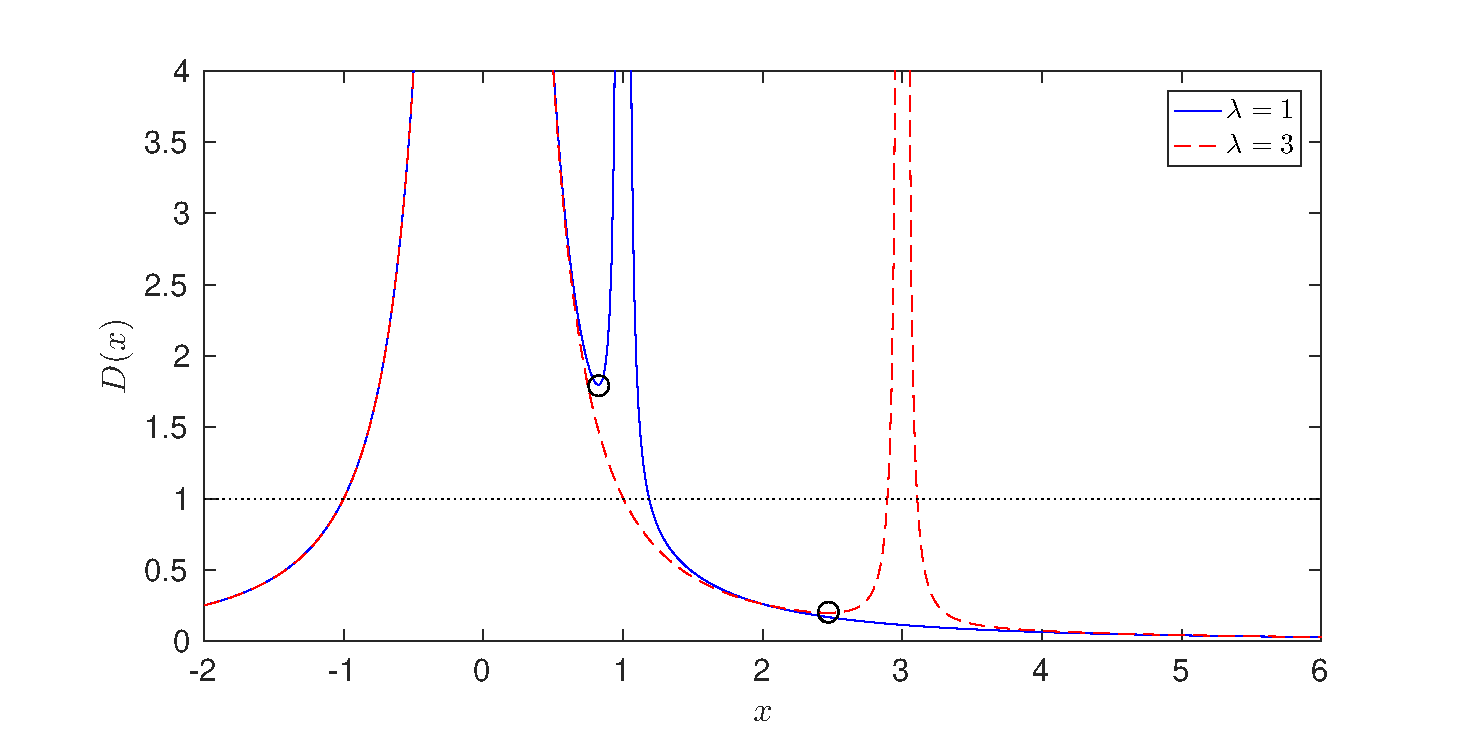
\includegraphics[width=12cm]{disp1.eps}
\caption{Graphical representation of the dispersion relation
  $D(x)=x^{-2}+\epsilon(x-\lambda)^{-2}=1$ for two different values of
  $\lambda$. Also marked in the figures are the local minima found
  in between the two singularities; if this minimum lies above the
  dotted line, then the solutions will be complex. }
\label{fig:disp}
\end{figure}

By defining the dimension-less quantities 
\begin{equation}
x:=\frac{\omega}{\back{\omega}{\text{p }}} \qc
\epsilon := \frac{\beam{\omega}{\text{p }^2}}{\back{\omega}{\text{p }^2}} 
=\frac{\beam{n}{}}{\back{n}{}} \qc \text{and}\quad
\lambda:=\frac{v_0k}{\back{\omega}{\text{p }}} 
\end{equation}
we can write the dispersion relation \eqref{eq2:disp} as
\begin{equation}
D(x)=\frac{1}{x^2}+\frac{\epsilon}{(x-\lambda)^2}=1.
\end{equation}
This is a function with two singularities $D(x)\to+\infty$, one at
$x=0$ and the other at $x=\lambda$. In between the singularities there
must be a local minimum. This is shown in \figref{fig:disp}. 
If that minimum is greater than $1$ the dispersion relation will have
a complex conjugate pair of solutions; obviously this happens when
$\lambda$ is small enough so that the two singularities are close
enough together. 
There will however \emph{always} be at least two real solutions, one
at $x<0$ and the other at $x>\lambda$. 

We can easily find this minimum by differentiation
\begin{equation}
\begin{aligned}
&0=\dv{D}{x}=-\frac{2}{x^3}-\frac{2\epsilon}{(x-\lambda)^3}\\
\stackrel{x\neq1, \lambda}{\Longleftrightarrow}&
-\epsilon x^3 = (x-\lambda)^3\\
\stackrel{x\in\R}{\Longleftrightarrow}&
-\epsilon^{1/3} x = (x-\lambda)\\
\Longleftrightarrow&
x_{\min}=\frac{\lambda}{1+\delta},
\end{aligned}
\end{equation}
where $\delta=\epsilon^{1/3}$. And the function value there is
\begin{equation}
D(x_{\min}) = \frac{(1+\delta)^2}{\lambda^2}
+\delta^3\qty[\lambda\frac{\delta}{1+\delta}]^{-2}
=\frac{(1+\delta)^2}{\lambda^2}\qty[1+\frac{\delta^3}{\delta^2}]
=\frac{(1+\delta)^3}{\lambda^2}.
\end{equation}
The condition for having complex solution is now easily formulated as
\begin{equation}
D(x_{\min}) > 1
\quad\Longleftrightarrow\quad
\lambda^2<(1+\delta)^3
\quad\stackrel{\lambda>0}{\Longleftrightarrow}\quad
\lambda<(1+\delta)^{3/2}.
\end{equation}
When this happens the solutions are called unstable, sine one of the
complex conjugate pair will exhibit exponential growth in wave
amplitude. 

\subsection*{Finding the complex solutions}
If we assume that $\epsilon\ll1$ ($\delta\ll1$), the condition above
for complex roots can be approximated as
\begin{equation}
\lambda\lesssim 1+\frac{3}{2}\delta.
\end{equation}

The solutions to this dispersion relation we can expressed as the
solutions to the quartic polynomial 
\begin{equation}
\frac{1}{x^2}-1+\frac{\epsilon}{(x-\lambda)^2}=0
\quad\stackrel{x\neq0, \lambda}{\Longleftrightarrow}\quad
(x-\lambda)^2(x-1)(x+1)-\epsilon x^2=0.
\end{equation}
We note that from the rational form, the reduced ($\epsilon=0$)
problem, we see that $x_0=\pm1$ is a reduced solution. We are only
interested in the solutions ``in between'' the two singularities,
meaning that we seek solutions $x\approx+1$.

We want to find the largest growth rate, i.e. largest imaginary part
of $\omega$. This occurs when the wave-plasma interaction is at its
largest, which heuristically is when the plasma (beam) velocity $v_0$
is close to the phase velocity $v_\text{phase}=\omega/k$ of the
wave. In other words $v_0/v_\text{phase}=\lambda/x$ should be
approximately 1. It is therefore \emph{reasonable to believe} that
$\lambda=1$ will maximize the imaginary part of $\omega$.
\footnote{I tried long and hard to find approximations for $x$ with a
  general $\lambda$, but so far no luck. }

The quartic polynomial therefore becomes
\begin{equation}
(x-1)^3(x+1)-\epsilon x^2=0.
\end{equation}
Since $x_0=1$ is a tripple root to the reduced problem, we have to
expand $x=x_0+\delta x_1+\order{\delta^2}$ with
$\delta=\epsilon^{1/3}$. To first order in $\delta$, we now get
\begin{equation}
\begin{aligned}
0=&(\delta x_1+\order*{\delta^2})^3(2+\order{\delta})
-\delta^3(1+\order{\delta})\\
=&(2x_1^3-1)\delta^3 + \order{\delta^4}
\end{aligned}
\end{equation}
We therefore see that
\begin{equation}
x_1 = \frac{\ee^{\ii 2\pi n/3}}{2^{1/3}}\qc n=-1, 0, 1;
\end{equation}
we are only interested in the complex solutions, which means that $n=\pm1$
We therefore have\footnotemark{}
\begin{equation}
x=1+\epsilon^{1/3}\frac{\ee^{\pm\ii2\pi/3}}{2^{1/3}}
+\order{\epsilon^{2/3}},
\end{equation}
meaning that the growth rate, for $\lambda=1$, is
\begin{equation}
\Im{\omega} =
\epsilon^{1/3}\frac{\sin(2\pi/3)}{2^{1/3}}+\order{\epsilon^{2/3}}
\approx 0.69\,\epsilon^{1/3}.
\end{equation}

\footnotetext{We do not have to worry that $\lambda=1$ and $x\approx1$
  will result in any problems in the rational form: 
  \[ 
  \frac{1}{x^2}-1+\frac{\epsilon}{(x-1)^2}
  =\frac{1}{1+\order{\delta}}-1+\frac{\delta^3}{(\order*{\delta})^2}
  =0+\order{\delta}.
  \]
  The rational function is really 0 for zeroth order in $\delta$. 
}



\section{Two-stream instability (kinetic theory)}
Here we will rederive the dispersion relation from the previous
problem using kinetic theory. We will only consider electrostatic
fields propagating along the $x$ direction, menaing that the 1D
Poisson-Vlasow equations are nessecary:
\begin{align}
& \pdv{f_\alpha}{t}+v\pdv{f_\alpha}{x}
-\frac{q_\alpha}{m_\alpha}\pdv{\varphi}{x}\pdv{f_\alpha}{v}=0\\
&\pdv[2]{\varphi}{x}=-\frac1\enull 
\sum_\alpha q_\alpha \int_{-\infty}^{\infty} [f_\alpha-F_{0\alpha}]\id{v}.
\end{align}
We are as always looking for perturbative solutions 
$f_\alpha=F_{0\alpha}+f_{1\alpha}$ and $\varphi=\varphi_0+\varphi_1$.
Like before the unperturbed solutions are static and uniform (in space
and time) meaning that we get, to linear order in the perturbations,
\begin{align}
& \pdv{f_{1\alpha}}{t}+v\pdv{f_{1\alpha}}{x}
+\frac{e}{\mee}\pdv{\varphi_1}{x}\pdv{F_{0\alpha}}{v}=0\\
&\pdv[2]{\varphi_1}{x}=\frac{e}{\enull}
\sum_\alpha \int_{-\infty}^{\infty} f_{1\alpha}(v) \id{v}.
\end{align}
Here we have also used the fact that we can disregard the ions, hence
all the charges are $q_\alpha=-e$ and $m_\alpha=\mee$.

Now Forier transform, according to \eqref{eq:Fourier}, the space and
time coordinates. Firstly 
\begin{equation}
\begin{aligned}
&-\ii\omega\tilde{f}_{\alpha}+v\ii k \tilde{f}_{\alpha}
+\frac{\ii ke}{\mee}\varphi_1\pdv{F_{0\alpha}}{v}=0\\
\quad\Longleftrightarrow\quad&
\tilde{f}_{\alpha}=\frac{ke}{\mee(\omega-vk)}\pdv{F_{0\alpha}}{v}
\tilde\varphi.
\end{aligned}
\end{equation}
Then
\begin{equation}
-k^2\tilde\varphi=\frac{k e^2}{\enull\mee} \sum_\alpha
\int_{-\infty}^{\infty}\pdv{F_{0\alpha}}{v}
\frac{\rd{v}}{(\omega-vk)}\tilde\varphi.
\end{equation}
By cleaning up a bit we get the dispersion relation
\begin{equation}
\begin{aligned}
-k=&\frac{e^2}{\enull\mee} \sum_\alpha
\int_{-\infty}^{\infty}\pdv{F_{0\alpha}}{v}
\frac{\rd{v}}{(\omega-vk)}\\
=&\frac{e^2}{\enull\mee} \sum_\alpha \qty{
\qty[\frac{F_{0\alpha}(v)}{(\omega-vk)^2}]_{v=-\infty}^\infty
-\int_{-\infty}^{\infty}F_{0\alpha}(v)
\frac{k\id{v}}{(\omega-vk)^2}
}.
\end{aligned}
\end{equation}
For the system to not have infinite energy, $F_{0\alpha}(v)\to0$ as
$v\to\pm\infty$, which cancels the first term after the integration by
parts. 

To continue further, we need to know more about $F_{0\alpha}$. In this
problem, we are given to assume
$F_{0\alpha}=n_{0\alpha}\delta(v-v_{0\alpha})$, where $\back{v}{0}=0$
and $\beam{v}{0}=v_0$. We can therefore write the dispersion relation
as
\begin{equation}
\begin{aligned}
1=&\frac{e^2\back{n}{0}}{\enull\mee} 
\int_{-\infty}^{\infty}\delta(v-0)
\frac{\id{v}}{(\omega-vk)^2}
+\frac{e^2\beam{n}{0}}{\enull\mee} 
\int_{-\infty}^{\infty}\delta(v-v_0)
\frac{\id{v}}{(\omega-vk)^2}\\
=&\frac{\back{\omega}{\text{p }}^2}{\omega^2}
+\frac{\beam{\omega}{\text{p }}^2}{(\omega-v_0k)^2},
\end{aligned}
\end{equation}
which is precisely the same dispersion relation as in the previous
problem.

We do not get any more information from \emph{this} approach with
kinetic theory, because we choose such a simple unperturbed
distribution function only containing \emph{one} velocity for each
species. The potential extra theoretical insights gained from using
kinetic theory comes from the fact that we, usually, have a
\emph{continuous spectrum} of velocities. 




%%%%%%%%%%%%%%%%%%%%%%%%%%%%%%%%%%%%%%%%%%%%%%%%%%%%%%%%%%%%%%%%%%%%%%
\end{document}%% ^ ^ ^ ^ ^ ^ ^ ^ ^ ^ ^ ^ ^ ^ ^ ^ ^ ^ ^ ^ ^ ^ ^ ^ ^ ^ ^
%%%%%%%%%%%%%%%%%%%%%%%%%%%%%%%%%%%%%%%%%%%%%%%%%%%%%%%%%%%%%%%%%%%%%%
%  LocalWords:  Debye Laramor quartic
